% TODO: Modifica immagine
\begin{figure}[h]
    \centering
    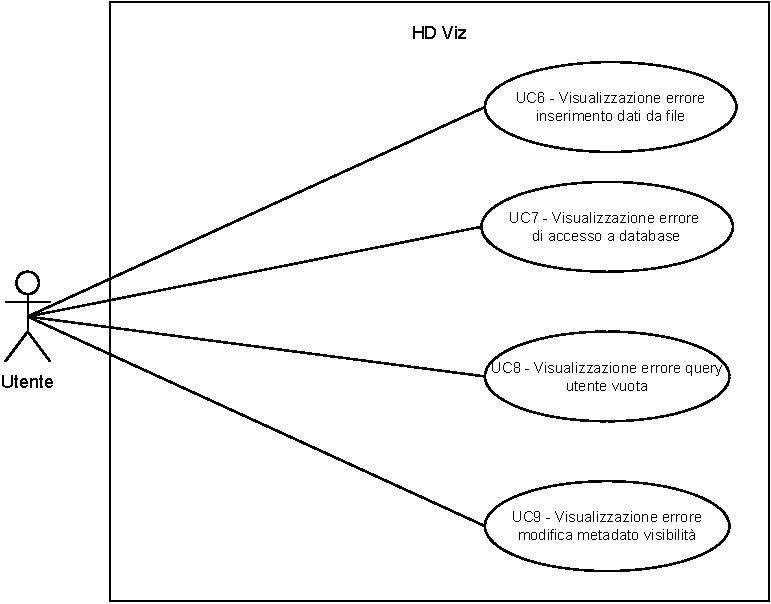
\includegraphics[width=0.7\textwidth]{diagrammi/UC_errori.pdf}
    \caption{Diagramma rappresentante gli use case degli errori}
    \label{fig:UC5}
\end{figure}

\subsection{UCW5 - Visualizzazione errore inserimento dati da file}
\label{sub:ucw5}
\begin{itemize}
    \item \textbf{Descrizione}: L'utente visualizza un messaggio di errore dopo aver caricato un file CSV non corretto 
    o vuoto;

    \item \textbf{Attore primario}: Utente;
    
    \item \textbf{Precondizione}:   L'utente carica un file CSV non corretto o vuoto (\hyperref[ssub:ucs1.2]{UCS1.2});

    \item \textbf{Postcondizione}:  Viene visualizzato un messaggio di errore relativo alla non correttezza del file 
    caricato;

    \item \textbf{Scenario principale}:
    \begin{enumerate}
        \item Viene visualizzato un messaggio d'errore relativo alla non correttezza del file caricato;
        \item L'utente conferma la presa visione dell'errore.
    \end{enumerate}

\end{itemize}